\documentclass{tufte-handout}

\title{More on Mathematical Induction}

\author{David Dobor}

\date{February 5, 2016} % without \date command, current date is supplied

%\geometry{showframe} % display margins for debugging page layout

\usepackage{graphicx} % allow embedded images
  \setkeys{Gin}{width=\linewidth,totalheight=\textheight,keepaspectratio}
  \graphicspath{{graphics/}} % set of paths to search for images
\usepackage{amsmath}  % extended mathematics
\usepackage{booktabs} % book-quality tables
\usepackage{units}    % non-stacked fractions and better unit spacing
\usepackage{multicol} % multiple column layout facilities
\usepackage{lipsum}   % filler text
\usepackage{fancyvrb} % extended verbatim environments
  \fvset{fontsize=\normalsize}% default font size for fancy-verbatim environments

% Standardize command font styles and environments
\newcommand{\doccmd}[1]{\texttt{\textbackslash#1}}% command name -- adds backslash automatically
\newcommand{\docopt}[1]{\ensuremath{\langle}\textrm{\textit{#1}}\ensuremath{\rangle}}% optional command argument
\newcommand{\docarg}[1]{\textrm{\textit{#1}}}% (required) command argument
\newcommand{\docenv}[1]{\textsf{#1}}% environment name
\newcommand{\docpkg}[1]{\texttt{#1}}% package name
\newcommand{\doccls}[1]{\texttt{#1}}% document class name
\newcommand{\docclsopt}[1]{\texttt{#1}}% document class option name
\newenvironment{docspec}{\begin{quote}\noindent}{\end{quote}}% command specification environment


\usepackage{listings}
\usepackage{color}

\definecolor{dkgreen}{rgb}{0,0.6,0}
\definecolor{gray}{rgb}{0.5,0.5,0.5}
\definecolor{mauve}{rgb}{0.58,0,0.82}

\lstset{frame=tb,
  language=matlab,
  aboveskip=3mm,
  belowskip=3mm,
  showstringspaces=false,
  columns=flexible,
  basicstyle={\small\ttfamily},
  numbers=none,
  numberstyle=\tiny\color{gray},
  keywordstyle=\color{blue},
  commentstyle=\color{dkgreen},
  stringstyle=\color{mauve},
  breaklines=true,
  breakatwhitespace=true,
  tabsize=3
}



\begin{document}

\maketitle% this prints the handout title, author, and date

\begin{abstract}
\noindent We have seen several examples of proofs using mathematical induction. Here we show two examples illustrating more creative uses of this proof technique. The first example has to do with a pie-fighting contest.\thanks{Adapted from Carmony, ``Odd Pie Fights'', \textit{Mathematics Teacher}, `79.} The second example is a misapplication of the principle of mathematical induction.  It ``proves'' that all horses are of the same color. 

\end{abstract}

\bigskip
\section{Odd Pie Fights}
\newthought{An odd number} of computer science students stand scattered around a yard, each student armed with a freshly baked apple pie.  The distance between any pair of students is distinct from the distance between any other pair. A whistle is suddenly blown and the pie throwing contest begins. Each contestant throws a pie at the contestant nearest to her. 

\bigskip
Use mathematical induction to show that there is at least one survivor. A survivor is a student who does not get hit by a pie.  

\bigskip
\textit{\underline{Proof:} } We will show that the following proposition $P(n)$ is true for all positive $n$:
\let\thefootnote\relax\footnotetext{Note that as $n$ runs through all positive integers, $2n + 1$ runs through all odd integers starting at 3 and greater. This is what we want -  we don't want to allow for a single pie-fighter; we need at least three - since we suspect that no sane person would want to engage into a pie fight with self. These are computer science  students, after all.}
 \begin{equation*}
 \begin{aligned}
P(n) = \{ \text{ There is a survivor whenever } 2n + 1  \text{ people standing at} \\ 
                                                       \text{mutually distinct distances throw pies at each other }\}
\end{aligned}
\end{equation*}


\newthought{\underline{Base Case:} $P(1)$ is true.} If $n = 1$, then we have $2n + 1 = 3$ people in the pie-fight. Let the three people be $A, B,$ and $C$. Let, without loss of generality, $A$ and $B$ be the closest pair.  Since the distances between all pairs  are different, we know that $C$ is closer to either $A$ or $B$. Let, again without loss of generality, $A$ be the closest guy to $C$. 

  What happens as the contest begins? $A$ and $B$ through pies at each other, and $C$ throws the pie at $A$. Thus we have the survivor, $C$. This proves the base case.
  
      

\newthought{\underline{Inductive Step:} If $P(k)$ is true, then $P(k+1)$ is true.} Assume that $P(k)$ is true for some odd integer $k > 3$. That is, we have at least one survivor when $2k + 1$ people pie-fight as described above. We must show that $P(k+1)$ is true. That is: we must show that there is at least one survivor whenever $2(k+1) + 1 = 2k + 3$ people pie-fight as described above.  

\bigskip
So suppose we have these $2k + 3$ people in the yard. Let $A$ and $B$ be the closest pair. When each person throws a pie, $A$ and $B$ throw pies at each other. 

\bigskip Now consider two cases: 1) Someone else throws a pie at either $A$ or $B$ and 2) No one else throws a pie  at either $A$ or $B$.
\newthought{\textit{Case 1: Someone else throws a pie at either $A$ or $B$.}} In this case \textit{at least } three pies are thrown at $A$ and $B$: 2 pies that they throw at each other and at least another pie that comes their way from somebody else. But this means that \textit{at most } $(2k+3) - 3 = 2k$ pies are thrown at the remaining $2k + 1$ people. But this guarantees that there is at least one survivor: there are fewer pies than people to be hit. 

\newthought{\textit{Case 2:  No one else throws a pie  at either $A$ or $B$.}} If nobody else throws a pie at either $A$ or $B$, then the proof is simpler. Consider removing $A$ and $B$ with their 2 pies from the $2k + 3$ people in the contest. We would be left with $2k + 1$ pie-fighting each other only. By the inductive hypothesis, there is at least one survivor amongst these $2k+1$ people. This person is also the survivor amongst the initial $2k + 3$ contestants (since $A$ and $B$ throw pies at each other).

\bigskip
This completes the proof. We proved the base case and we proved the inductive step using a proof by cases. From the principle of mathematical induction it follows that $P(n)$ is true for all positive integers $n$. 

\bigskip
Notice that the conclusion we reached here would be false if the contest set-up were the same as before but we had an even number of people in the yard. Can you see why is it possible for everyone to be hit with a pie in this case?
%\begin{marginfigure}
%  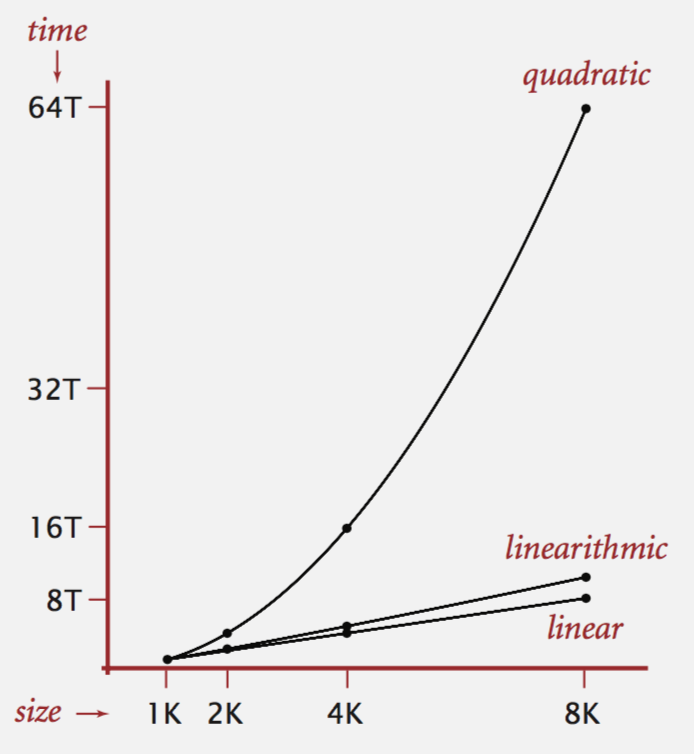
\includegraphics{graph}
%  \caption{A $O(n^2)$ algoritm scales horribly.}
%\end{marginfigure}

\section{Are All Horses Purple?}

\newthought{Our next example } is of misuse of mathematical induction.  We look at how mathematical induction can be used to ``prove'' that all horses are of the same color.

\bigskip
\newthought{Theorem: } All horses are of the same color.

\textit{\underline{Proof:} } \marginnote{Note that we can not make the sentence `All horses are of the same color' our predicate. Why not? Because we need the predicate to depend on $n$ on which to induct. }
Let our predicate be
 \begin{equation*}
 \begin{aligned}
P(n) = \{ \text{ In any set of } n \geq 1  \text{ horses, the horses are all the same color.} \} %\\ 
                                                      % \text{mutually distinct distances throw pies at each other }\}
\end{aligned}
\end{equation*}

\newthought{\underline{Base Case:} $P(1)$ is true.} I see one horse, it's of some color, say purple. It is trivially true that all horses in this set consisting of just one horse are of the same color. Base case proved.

\newthought{\underline{Inductive Step:} Assume $P(k)$ is true and show that then $P(k+1)$ is also true.} 
 Consider a set of $k+1$ horses:
$$
\{ H_1, H_2, \cdots, H_{k}, H_{k+1} \}
$$
How can we see that, given our assumption that any subset of $k$ horses of this set of $k+1$ horses are of the same color, \textit{all} these $k+1$ horses have to be of the same color? Why do $H_1$ and $H_{k+1}$ have to be of the same color, for example\marginnote{Of course, there is nothing special about $H_1$ and $H_{k+1}$. The argument that follows holds true for any pair of horses.}? 

\bigskip
To see this, note that by assumption
 \begin{equation*}
 \begin{aligned}
\{ H_1, H_2, \cdots, H_{k} \}  \text{ are all the same color.} 
\end{aligned}
\end{equation*}
and
\begin{equation*}
 \begin{aligned}
\{ H_2, H_3, \cdots, H_{k+1} \}  \text{ are also all the same color.}
\end{aligned}
\end{equation*}

\bigskip
Then color($H_1$) has to be the same as color($H_{k+1}$) since  

\begin{equation}
\text{color}(H_1) = \text{color}( H_2, H_3, \cdots, H_k)                                           
\end{equation}
and
\begin{equation}
\text{color}(H_{k+1}) = \text{color}( H_2, H_3, \cdots, H_k)                                           
\end{equation}

\bigskip
Putting (1) and (2) together gives that 
\begin{equation*}
\text{color}(H_{k+1}) = \text{color}(H_1)                                       
\end{equation*}

This completes the proof by mathematical induction. We've followed the proof template we've always used, one that we believe produces correct proofs.  Yet we somehow are unable to have faith the claim that all horses are of the same color. 

 \bigskip
 So what gives? The principle of mathematical induction or your prior experience with the world telling you that not all horses are of the same color? 


\end{document}


There are plenty of opportunities for making errors when using mathematical induction. Here is an example: we ``prove'' that all horses are of the same color? 

















